\documentclass[12pt]{article}

\usepackage{array}
\usepackage{setspace}
\usepackage{xspace}
\usepackage{url}
\usepackage{graphicx}
\usepackage{tipa}
\usepackage[colon,round]{natbib}

\usepackage{amsmath}
\usepackage{amsopn}
\usepackage{amssymb}
\usepackage{amsfonts}

\usepackage{listings}
\usepackage{color}
\usepackage{xcolor}
\usepackage[font=footnotesize,labelfont=bf]{caption}

\usepackage{hyperref}
\hypersetup{
  colorlinks,
  citecolor=black,
  filecolor=black,
  linkcolor=black,
  urlcolor=black
}

\usepackage{fancyvrb}
\usepackage{tgcursor}
\fvset{fontsize=\footnotesize}

\definecolor{dkgreen}{rgb}{0,0.6,0}
\definecolor{gray}{rgb}{0.5,0.5,0.5}
\definecolor{mauve}{rgb}{0.58,0,0.82}
\definecolor{lightgray}{rgb}{0.95, 0.95, 0.95}

\lstset{%
  language=perl,
  basicstyle=\footnotesize\ttfamily\setstretch{0.5},
  columns=fullflexible,
  stringstyle=\color{mauve},
  aboveskip=1mm,
  belowskip=1mm,
  showstringspaces=false,
  numbers=none,
  commentstyle=\fontseries{lc}\selectfont\itshape\color{gray}\scriptsize,
}

% bug: arrow is not syntax-highlighted
\lstset{emph={%
    START,FINAL,<-%
  },emphstyle={\color{red}}%
}%

\newcommand{\yellowlisting}[1]{%
  \lstinputlisting[backgroundcolor=\color{yellow!20}]{#1}}

\usepackage{verbatim}
\usepackage{alltt}

\usepackage[framemethod=TikZ, outerlinewidth=0, backgroundcolor=yellow!10,
  innerleftmargin=7pt, innerrightmargin=7pt,%
  innertopmargin=4pt, innerbottommargin=4pt,%
  roundcorner=10pt, leftmargin=10, rightmargin=10]{mdframed}

\usepackage[upright]{fourier}
\usepackage{tikz}
\usetikzlibrary{shapes,arrows,calc,positioning,shadows}

\newcommand{\hyp}{\texttt{hyp}\xspace}
\newcommand{\code}[1]{\texttt{#1}}
\newcommand\todo[1]{\textcolor{red}{TODO: #1}}

% \newcommand{\hypdraw}{\texttt{hypdraw}\xspace}
% \newcommand{\hypcompose}{\texttt{hypcompose}\xspace}
\newcommand{\hypdraw}{\texttt{HypDraw}\xspace}
\newcommand{\hypcompose}{\texttt{HypCompose}\xspace}

\newcommand{\vtheta}{\boldsymbol{\theta}}
\newcommand{\ptheta}{p_{\vtheta}}
\newcommand{\utheta}{u_{\vtheta}}

\newcommand\argmin{\operatornamewithlimits{argmin}}
\newcommand\argmax{\operatornamewithlimits{argmax}}

\renewcommand{\eqref}[1]{Equation~\ref{eq:#1}}
\newcommand{\tabref}[1]{Table~\ref{tab:#1}}
\newcommand{\secref}[1]{Section~\ref{sec:#1}}
\newcommand{\figref}[1]{Figure~\ref{fig:#1}}

\let\cite\citep    % parens
\let\newcite\citet % no parens

\renewcommand\floatpagefraction{.8}
\renewcommand\topfraction{.9}
\renewcommand\bottomfraction{.9}
\renewcommand\textfraction{.1}
\setcounter{totalnumber}{50}
\setcounter{topnumber}{50}
\setcounter{bottomnumber}{50}

% name, caption, img width
% scales the image width
\newcommand{\exampleb}[3]{
  \begin{table}[!tbp]
    \centering
    \begin{tabular}[h]{ l }\hline
      \begin{minipage}{\textwidth}
        \lstinputlisting{fig/#1.hyp}
      \end{minipage}
      \\
      \includegraphics[width=#3\columnwidth]{fig/#1.pdf} \\\hline
    \end{tabular}
    \caption{#2}
    \label{tab:#1}
  \end{table}
}

% args: name, caption, fig width, move fig to left
\newcommand{\examplecols}[4]{
  \begin{table}[!tbp]
    \centering
    \begin{tabular}[t]{p{0.65\textwidth} p{0.3\textwidth}}\hline
      \vspace{-3pt}
      \lstinputlisting{fig/#1.hyp}
      &
      \vspace{-5pt}
      \begin{tabular}[t]{l}%
        \hspace{-#4}
        \includegraphics[width=#3\columnwidth]{fig/#1.pdf}\\
      \end{tabular}%
      \\\hline
    \end{tabular}
    \caption{#2}
    \label{tab:#1}
  \end{table}
}

% args: name, caption, fig width, lower figure
\newcommand{\example}[4]{
  \begin{table}[!tbp]
    \centering
    \begin{tabular}{ l }\hline
      \lstinputlisting{fig/#1.hyp}
      \vspace{#4}
      \\
      \includegraphics[width=#3\columnwidth]{fig/#1.pdf} \\\hline
    \end{tabular}
    \caption{#2}
    \label{tab:#1}
  \end{table}
}

\title{Tutorial: The \hyp{} hypergraph toolkit}

\author{
  Markus Dreyer\\
  SDL\\
  6060 Center Drive Suite 150\\
  Los Angeles, CA 90045\\
  \url{mdreyer@sdl.com}
  \and
  Jonathan Graehl\\
  SDL\\
  6060 Center Drive Suite 150\\
  Los Angeles, CA 90045\\
  \url{graehl@sdl.com}
}
\date{\today}

%%%%%%%%%%%%%%%%%%%%%%%%%%%%%%%%%%%%%%%%%%%%%%%%%%%%%%%%%%%%%%%%%%%%%%%%%%%%%%%%

\begin{document}

\maketitle

\begin{abstract}
  We present \hyp, a general toolkit for the representation,
  manipulation, and optimization of weighted hypergraphs. Finite-state
  machines are modeled as a special case.
\end{abstract}

\tableofcontents

\section{Introduction}

The \hyp{} toolkit provides data structures and algorithms to process
weighted directed hypergraphs.

Such hypergraphs are important in natural language processing and
machine learning. Their use arises naturally in parsing
\cite{klein_parsing_2005, huang_better_2005}, syntax-based machine
translation and other tree-based models, as well as in logic
\cite{gallo_directed_1993} and weighted logic programming
\cite{eisner_dyna:_2011}.

We present a toolkit for the representation and manipulation of
weighted directed hypergraphs. It provides data structures for
hypergraphs as well as many algorithms, such as \code{compose},
\code{project}, \code{invert}, the shortest path algorithm, the inside
and outside algorithm, and more. In addition, it provides
functionality to optimize hypergraph feature weights from training
data.

\section{Definitions}\label{sec:definitions}
A weighted directed hypergraph (henceforth just \textit{hypergraph})
is a pair $H=\langle V,E\rangle$, where $V$ is a set of vertices and
$E$ a set of edges. Each edge (also called \textit{hyperedge}) is a
triple $e=\langle T(e), h(e), w(e) \rangle$, where $T(e)$ is an
ordered list of tails (i.e., source vertices), $h(e)$ is the head
(i.e., target vertex) and $w(e)$ is the semiring weight of the edge
(see \figref{hyperarc}). Semirings are described in
\secref{semirings}.

\begin{figure}[t]
  \centering
  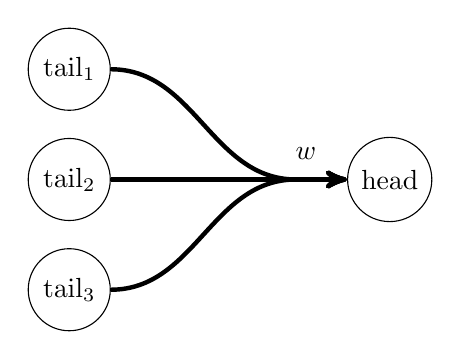
\begin{tikzpicture}[
      > = stealth',
      node distance = 1.4cm
    ]
    \tikzstyle{my line} = [->, ultra thick]
    \tikzstyle{main node} = [circle, draw]
    \node[main node] (A) {tail$_1$};
    \node[main node] (B) [below of=A] {tail$_2$};
    \node[main node] (C) [below of=B] {tail$_3$};
    \node[main node] (H) [right=3cm of B] {head};
    \node (H0) [left=0.4cm of H] {};
    \draw[my line] (A) to[out=0,in=180] (H0) to[out=0,in=180] (H);
    \draw[my line] (B) to (H);
    \draw[my line] (C) to[out=0,in=180] (H0) to[out=0,in=180] (H);
    \node (w) [above=0cm of H0] {$w$};
  \end{tikzpicture}
  \caption{An arc leading from three tail states to a head state,
    with weight $w$.}
  \label{fig:hyperarc}
\end{figure}

We regard hypergraph as \textit{automata} and call the vertices
\textit{states} and edges \textit{arcs}. We add an optional start
state $S\in V$ and a final state $F\in V$.

The set of incoming arcs into a state $s$ is called the
\textit{Backward Star} of $s$, or short, $\mathrm{BS}(s)$. Formally,
$\mathrm{BS}(s) = \{a\in E : h(a) = s\}$.

A \textit{path} $\pi$ is a sequence of arcs $\pi = (a_1 \dots a_k) \in
E^*$ such that $\forall a \in \pi, \forall t \in T(a), (\exists a' \in
\pi : h(a')=t) \lor \mathrm{BS}(t)=\emptyset$. In words, each tail
state $t$ of each arc on the path must be the head of some arc on the
path, unless $t$ has no incoming arcs (i.e., is a leaf state). The
rationale is that each tail state of each arc on the path must be
\textit{derived}, by traveling an arc that leads to it, or given as an
\textit{axiom}.  If the hypergraph has a start state, the first tail
of the first arc of any path must be the start state. The head of the
last arc must always be the final state, $h(a_k)=F$.

The hypergraphs we consider, in which each arc has exactly one head,
have been called \textit{B-hypergraphs} \cite{gallo_directed_1993}, as
opposed to the more general version in which multiple head states are
allowed.

\section{Representing hypergraphs}

\hyp uses a simple text format for hypergraphs, which makes it easy to
write down and construct toy hypergraphs and play with them.

\subsection{Constructing a one-arc toy hypergraph}

Let's construct our first hypergraph! It has only a single arc, which
is written as \texttt{0 <- 1 2 3 / 0.693}, denoting the head state 0,
the tail states 1, 2, 3, and the weight 0.693.  The text and visual
representations are shown in \tabref{one_arc}.  Each state has an ID
(see number in circle). State 0 is the final state and is marked as
such: \texttt{FINAL <- 0}. Similar to finite-state machine convention,
the final state is drawn as a double circle. The small gray numbers
denote the ordering of the tails of the arc. We draw any leaf node
gray.\footnote{This is in analogy to graphical models, where
  \textit{observed} nodes are drawn gray, denoting that they do not need
  to be derived or inferred.}  The visual representation has been
created with the \hypdraw command.  \exampleb{one_arc}{The text and
  visual representation of a simple hypergraph with only a single
  arc.}{0.25}

That's nice, but usually we also need labels. As described in
\secref{definitions}, our hypergraph arcs do not have labels, but
states do. \tabref{one_arc_labels} shows how labels are added. The
result is similar to the typeset example in \figref{hyperarc}.

\exampleb{one_arc_labels}{The same hypergraph as in \tabref{one_arc},
  but here the states are labeled. For simplicity, we leave out the
  state IDs of labeled states in the visual representation.}{0.25}

\subsection{Trees and forests}

Hypergraphs can represent trees and (packed or non-packed) forests,
but they can also---as special cases---represent strings, lattices, or
finite-state machines. Let's start with trees and forests; we'll come
back to strings, lattices, etc., later.

\subsubsection{Trees}\label{sec:tree}

A tree is a typical, simple hypergraph. \tabref{tree} shows a labeled,
unweighted tree and the corresponding text format.
\examplecols{tree}{A simple tree.}{0.65}{5.3cm} Again, the gray
numbers 1, 2, 3, \dots in the figure denote the ordering of the tails
of an arc. State IDs are not shown wherever labels are given.  The
text format contains one arc per line. Each arc has the following
format:
\begin{verbatim}
    head <- tail1 tail2 ... tailn
\end{verbatim}
Each head or tail state consists of a state ID and a label,
\code{ID(label)}. The label is enclosed in double-quotes if it is
lexical (i.e., a word).  Each arc may have a weight (optional):
\begin{verbatim}
head <- tail1 tail2 ... tailn / weight
\end{verbatim}
A weight is typically a negative log number (i.e., the cost of the
arc). A final state \code{n} is marked as \code{FINAL <- n}.

\subsubsection{Reducing redundancy in the text format}

To reduce redundancy, we can leave out labels wherever they can be
inferred:
\yellowlisting{fig/sticks_less_labels1.hyp}

To further reduce redundancy, we can also leave out state IDs wherever
they can be inferred:
\yellowlisting{fig/sticks_less_labels2.hyp}

We can leave out all state IDs. In the above example, however, states
\code{1} and \code{5} both have the same label \code{NP}, so if we
just leave out the state labels these states will be seen as
identical. We give them different labels and can leave out all state
IDs, see \tabref{sticks_no_ids}.

\examplecols{sticks_no_ids}{Leaving out all state IDs in the text
  format.}{0.68}{5.7cm}

\subsubsection{Forests}

A forest is a hypergraph that contains more than one tree. The forest
may be \textit{packed}, in which case the trees share substructure,
just like strings in a lattice. We can turn the tree from
\secref{tree} into a forest by adding some arcs, see \tabref{forest}.
\example{forest}{A packed forest.}{0.95}{-1.7cm}
That forest represents two interpretations of the sentence, where he
(1) eats rice that has sticks or (2) eats rice using sticks as a tool.

\subsection{Constructing strings, lattices, and FSMs}

\subsubsection{Strings}

In the finite-state world, a string is often encoded as a simple,
flat-line finite-state machine.  It is a left-recursive split of the
string as \code{( ( ( He ) eats )
  rice )}, i.e., we first have ``He'', then combine it with ``eats'',
then combine the result with ``rice'' to accept the whole string, see
\tabref{sent_fst}.

\examplecols{sent_fst}{A one-sentence finite-state machine. The text
  here is in the OpenFst text format.}{0.4}{6cm}

We can do something similar using hypergraphs, see \tabref{sent1}.
\examplecols{sent1}{A sentence expressed as a simple
  hypergraph.}{0.4}{5cm} All leaves in this lattice-like hypergraph are
``axioms''; they are given.  The hypergraph can be traversed bottom-up
as follows: First we have (start) state 0 and the ``he'' state. Given
those, we reach state 1. Given state 1 and the axiom ``eats'' we reach
state 2. Given state 2 and axiom ``rice'', we reach final state
3. (The start state 0 is optional here.)  The figure can be understood
as an unusual way to draw a lattice/finite-state machine: The arc from
0 to 1 has its label drawn as a balloon hanging off the
arc. Similarly, for the arcs \code{1 -> 2} and \code{2 -> 3}.

\subsubsection{Lattices and general finite-state machines}

We can add more arcs to the string to turn it into a lattice, see
\tabref{lattice}.  \examplecols{lattice}{A simple lattice
  hypergraph.}{0.4}{5cm}

Or we can turn it into a general finite-state machine by adding a loop
arc: \yellowlisting{fig/loop.hyp}
% Not drawn correctly:
% \examplecols{loop}{A simple finite-state machine with a loop.}{0.6}{5cm}

We call these special, restricted hypergraphs, in which each arc has a
structural tail state followed by a lexical tail state,
\textit{regular} or \textit{finite-state} hypergraphs.

Note to avoid confusion: An arc like \code{2 <- 1 (``likes'')} has two
tails: State 1, for which no label is specified, and the state with
label \code{(``likes'')}, for which no state ID is specified.

\subsection{Transducers}

Any (leaf) state may have ``rewrite information'', i.e., a specific
output label, in addition to the input label. For example, the
following machine rewrites ``he eats rice'' to ``he ate rice''; it is
a finite-state transducer (in \hyp hypergraph format):
\yellowlisting{fig/fst.hyp}

Note that general hypergraphs (trees, forests, etc.) may have output
labels as well. The following hypergraph rewrites ``he eats rice with
sticks'' to ``he ate pasta''; it also parses the input string into a
structure that (unlike the example above) is not just left-recursive:
\yellowlisting{fig/tree_transduce.hyp}

Special symbols like epsilon, phi, rho, sigma are written with
brackets, as \code{<eps>}, \code{<phi>}, \code{<rho>}, \code{<sigma>}.

When a state has no explicit output label the output label is assumed
to be similar to the input label---a convention from the finite-state
world.

In order to rewrite a string, we compose it with the input (see
\secref{compose}). Our code uses a generalized composition algorithm
that can compose a (weighted) general hypergraph with a (weighted)
finite-state hypergraph. It is a generalization of the Earley
algorithm, see \cite{earley_efficient_1970},
\cite{stolcke_efficient_1995}, \cite{ eisner_compiling_2005},
\cite{dyer_formal_2010}. Like with finite-state machines, we can
project to the output after composing, to obtain the resulting
acceptor (see \secref{invert-project}).

\subsection{Semirings and features}\label{sec:semirings}

Each hypergraph uses a particular semiring. Semirings are used to
specify the type of the weights and define how weights are added and
multiplied.  We provide the two standard semirings log and Viterbi, as
well as the expectation semiring \cite{eisner-2002-acl-fst}. The
semiring can be specified when using the command line tools (see
below) or when constructing a hypergraph in C++.

Using the expectation semiring enables us to place features on the
arcs. Example:

\begin{verbatim}
4(V) <- 11("eats" "ate") / 3.2[0=3.2,8=3.2]
\end{verbatim}

where the arc has weight 3.2 and feature 0 and feature 8 fire once,
respectively (so their expected values are both 3.2).

We also added a new semiring called feature semiring, which behaves
exactly like the Viterbi semiring but allows for a feature vector on
each arc, like the expectation semiring.

Using the expectation or the feature semiring, we can keep track of
what features fire on what arcs when we compose several hypergraphs
(or perform other operations). Using standard algorithms that we
implemented (e.g., the inside-outside algorithm, see below), it is
possible to train hypergraphs as a CRF (see \secref{optimize}), for
example. See \secref{inside} for an example that demonstrates the
behavior of different semirings.

\section{Using Hypergraph command line tools}

We created various command line tools that process and manipulate
hypergraphs. They accept hypergraph input in the text format described
above. The command line tools can be used to compose, concatenate,
invert, create unions, extract k-best paths, run the inside algorithm,
etc.

\subsection{HypCompose}\label{sec:compose}

As an example, consider composing a CFG hypergraph with an input
sentence hypergraph:

\begin{mdframed}\footnotesize\begin{alltt}
$ cat cfg.hyp
\input{fig/cfg_include.hyp}
$ cat sent.hyp
\input{fig/sent1.hyp}
$ \textbf{HypCompose} cfg.hyp sent.hyp
\end{alltt}\end{mdframed}

\noindent The result is a packed parse forest, see
\tabref{compose_result}.
\example{compose_result}{Composition result: A packed forest.}{0.8}{0.3cm}

\subsubsection{Natural language parsing}

Note that we can do weighted lattice parsing: A weighted context-free
grammar (CFG) can be encoded as a hypergraph and can be composed with
finite-state input (e.g., a string or a weighted lattice), using our
composition algorithm. The result is the parse of the whole input
structure. Note, however, that the CFG composition algorithm in \hyp
currently does not perform pruning and can therefore only used with
small grammars. If both hypergraphs are \textit{finite-state},
however, \code{HypCompose} switches to a fast finite-state composition
algorithm.

\subsubsection{Hypergraph rescoring}

We can also rescore a weighted hypergraph by composing (or similarly,
intersecting) with a finite-state machine, e.g., a language model.

\subsection{HypPruneToBest, HypBest}\label{sec:hgbest}

To get an $n$-best list from any hypergraph, use \code{HypBest}. For
example, the two entries in the composition result
(\tabref{compose_result}) are:

\begin{mdframed}\footnotesize\begin{alltt}
$ HypCompose cfg.hyp sent.hyp | \textbf{HypBest} --num-best=2
  n=1 2.07944 "he" "eats" "rice"
  n=2 3.68888 "he" "eats" "rice"
\end{alltt}\end{mdframed}

To print the best tree, use \code{HypPruneToBest}. Example:
\begin{mdframed}\footnotesize\begin{alltt}
$ HypCompose cfg.hyp sent.hyp | \textbf{HypPruneToBest}
  FINAL <- 0(S)
  0(S) <- 1(NP) 2(VP) / 0.182322
  1(NP) <- 5(N) / 0
  2(VP) <- 3(V) 4(NP) / 0
  3(V) <- 8("eats") / 0
  4(NP) <- 7(N) / 0
  5(N) <- 6("he") / 0.693147
  7(N) <- 9("rice") / 1.20397
\end{alltt}\end{mdframed}

Remember that all arc weights are interpreted as negative log numbers,
i.e., costs, and the best parse is the one with the lowest cost.

\subsection{HypInside}\label{sec:inside}

The inside algorithm computes the cost of reaching each state starting
from the leaves.

In \tabref{compose_result}, for example, the final state $0$ can be
reached via two different paths, which have weights $2.07944$ and
$3.68888$, respectively. The sum in negative log space is
$-\log(\exp(-2.07944) + \exp(-3.68888))=1.897117$. \code{HypInside},
called on the hypergraph from \tabref{compose_result}, gives exactly
that result for state $0$ and lists the costs for reaching the other
states as well:

\begin{mdframed}\footnotesize\begin{alltt}
$ \textbf{HypInside} foo.hyp
  0       1.89712
  1       1.20397
  2       0.693147
  3       0.693147
  4       0
  ...
\end{alltt}\end{mdframed}

If the Viterbi semiring is used, then the costs of any alternative
paths are not added up, but the best among them is picked, so we
have:

\begin{mdframed}\footnotesize\begin{alltt}
$ HypInside \textbf{--arc-type=viterbi} foo.hyp
  0       2.07944
  1       1.20397
  2       0.693147
  3       0.693147
  4       0
  ...
\end{alltt}\end{mdframed}

The feature semiring computes arc weights just like the Viterbi
semiring, but in addition it accumulates features, where feature
values are not in log space. Consider the hypergraph in
\tabref{compose_result}, but with real-valued features added on some
arcs:

\begin{mdframed}\footnotesize\begin{alltt}
$ cat feats.hyp
\input{fig/compose_result_feature.hyp}
\end{alltt}\end{mdframed}

On the first arc, feature $0$ fires $1.3$ times and feature $1$ fires
twice. The output of \code{HypInside} looks like the Viterbi result
above, but with the accumulated feature vectors added:

\begin{mdframed}\footnotesize\begin{alltt}
$ HypInside \textbf{--arc-type=feature} feats.hyp
  0       2.07944[0=1.3,1=6]
  1       1.20397[1=4]
  2       0.693147
  3       0.693147
  4       0
  ...
\end{alltt}\end{mdframed}

If the expectation semiring is used on a hypergraph with features, the
inside algorithm computes the expected value of each feature for each
state. For the final state, we get the expected value of each feature
in the overall hypergraph.\footnote{This property of the expectation
  semiring is remarkable because the feature expectations can otherwise
  only be computed by running the inside \textit{and} the outside
  passes. Note, however, that the expectation semiring accumulates
  feature expectations in all its inside weights, so those vectors
  become denser for states closer to the final state. It is often more
  efficient to compute feature expectations by running the inside and
  outside passes in the log semiring, then passing over the hypergraph
  again and accumulating the feature expectations in just one vector. We
  use this method in \code{Hypergraph/FeatureExpectations.hpp}.}

For the expectation semiring, each arc weight is a tuple of the weight
$w$ and the feature vector $v$ times $w$
\cite{eisner-2002-acl-fst}. We take the negative log of $w$ and of
$vw$. For example, in the following example, the first arc has
$w=5\slash 6$ and $v=[1.3, 2]$, so $vw=[1.08,1,67]$. The numbers on
the arc are the negative log of these, so we have (rounded)
$0.1823[0=-0.0800,1=-0.5108]$, see here:

\begin{mdframed}\footnotesize\begin{alltt}
$ cat expectation.hyp
\input{fig/compose_result_expectation.hyp}
\end{alltt}\end{mdframed}

\noindent\code{HypInside} lists the (negative log of the) feature expectations
at each state:

\begin{mdframed}\footnotesize\begin{alltt}
$ HypInside --arc-type=expectation expectation.hyp
  0       1.89712[0=1.60943,1=0.510826,2=2.59026]
  1       1.20397[1=-0.182322]
  2       0.693147
  3       0.693147
  4       0
  ...
\end{alltt}\end{mdframed}

Observe that the inside cost of the final state $0$ is listed as
$1.89712$, i.e., $-\log(0.15)$, just like when the log semiring is
used (see above). The expected value of feature $0$ is listed as
$-1.60943$, i.e., $-\log(0.2)=-\log(0.125 \times 1.3 + 0.025 \times
1.5)$, because that feature fires $1.3$ times on the best path and
$1.5$ times on the other path.

\subsection{HypInvert, HypProject}\label{sec:invert-project}

The \code{invert} operation swaps input and output labels of all arcs.
For example, the following toy transducer changes \textit{eat} or
\textit{sleep} to their past tense forms (while accepting any other
word without change via the special \code{<rho>} symbol):

\begin{mdframed}\footnotesize\begin{alltt}
$ cat past_tense.hyp
\input{fig/past_tense.hyp}
\end{alltt}\end{mdframed}

\noindent The inverted version changes those past tense forms back to
\textit{eat} or \textit{sleep}:

\begin{mdframed}\footnotesize\begin{alltt}
  cat past_tense.hyp | \textbf{HypInvert}
\input{fig/past_tense_inverted.hyp}
\end{alltt}\end{mdframed}

The \code{project} operation projects to the output labels by removing
the input labels, or vice versa. This is often useful for obtaining
the output after composing. Example:

\begin{mdframed}\footnotesize\begin{alltt}
$ cat sent.hyp
\input{fig/sent2.hyp}
$ HypCompose sent.hyp past_tense.hyp | \textbf{HypProject}
\input{fig/he_ate_rice.hyp}
\end{alltt}\end{mdframed}

\subsection{HypUnion}

The \code{HypUnion} executable takes the union of two or more
hypergraphs. The union operation implements an OR logic, so that in
the resulting hypergraph, one can follow the paths of any of the input
hypergraphs. Example:

\begin{mdframed}\footnotesize\begin{alltt}
$ cat ab.hyp
\input{fig/ab.hyp}
$ cat kl.hyp
\input{fig/kl.hyp}
$ cat xyz.hyp
\input{fig/xyz.hyp}
$ HypUnion ab.hyp kl.hyp xyz.hyp
\end{alltt}\end{mdframed}

The result is shown in \tabref{union_result}.
\examplecols{union_result}{Union result.}{0.4}{1.7cm}

\subsection{HypConcat}

The \code{HypConcat} concatenates two or more hypergraphs. If you
use \code{HypConcat} instead of \code{HypUnion} in the example above,
you obtain the output shown in \tabref{concat_result}.
\examplecols{concat_result}{Concat result.}{0.4}{1.7cm}

\subsection{Other \hyp executables}

The \hyp toolkit also provides the following executables, in addition
to the ones discussed above:

\begin{itemize}
\item \code{HypComplement} creates the complement of an unweighted
  finite-state hypergraph
\item \code{HypConvertStrings} converts string input into string
  hypergraphs (i.e., hypergraphs like the one shown in
  \tabref{sent1})
\item \code{HypDeterminize} determinizes a finite-state hypergraph
  (currently only unweighted acceptors allowed)
\item \code{HypDraw} draws a hypergraph in \code{dot} format (see the
  figures in this tutorial)
\item \code{HypEmpty} decides if a hypergraph is empty, i.e., has no
  valid paths
\item \code{HypGetString} prints the string contained in a one-path
  hypergraph
\item \code{HypPrune} prunes away all unreachable arcs of a hypergraph
\item \code{HypReverse} reverses a hypergraph
\item \code{HypReweight} modifies arc weights of a hypergraph
\item \code{HypSamplePath} generates sample paths from a hypergraph
\end{itemize}

\section{Using the C++ API}

We now describe basic usage of the C++ API. See also the complete
example code in \texttt{HypDemo/src/HypDemo.cpp}.

The full API documentation can be generated using \code{doxygen doxygen/xmtDoxy.conf}.

\subsection{Creating a forest}\label{sec:creating-forest}

The following code creates a toy forest hypergraph:

\lstset{
  language=C++,
  numbers=left
}
\yellowlisting{CreateForest.hpp}

The code first creates a vocabulary and adds a few terminal symbols
and a nonterminal symbol. It creates the hypergraph and sets its
vocabulary. It then adds states and arcs where each arc has a head,
tails, and a weight. It then sets the final state.

\subsection{Hypergraph properties}

Each hypergraph object has properties, expressed as bits in a 64-bit
number, see \texttt{Hypergraph/Properties.hpp}. These can describe
properties of the hypergraph at any point in time, e.g.,
\texttt{kFsm}, which is on by default until non-finite-state arcs are
added, or \texttt{kCfg}. Other properties act as policies that control
behavior such as an arc storage discipline. We now describe two of
these policies.

\subsubsection{Arc storage}

By default, each hypergraph object keeps track of incoming and
outgoing arcs per state. For large hypergraphs, one might want to save
memory by storing only incoming or only outgoing arcs. Typically, if
the hypergraph represents a regular language (e.g., string, lattice)
just storing outgoing arcs are sufficient. For context-free languages
(e.g., tree, forest) incoming arcs are sufficient for running most
algorithms on the hypergraph. These property bits can be set in the
constructor:

\lstset{ backgroundcolor=\color{yellow!20}, numbers=none }
\begin{lstlisting}
  MutableHypergraph<Arc> hyp1(kStoreInArcs);
  MutableHypergraph<Arc> hyp2(kStoreOutArcs);
  MutableHypergraph<Arc> hyp3(kStoreInArcs | kStoreOutArcs); // default
\end{lstlisting}

\subsubsection{Canonical lexical states}

Another useful property is \texttt{kCanonicalLex}. It has the effect
that any terminal label will be associated with one particular
(``canonical'') state in the hypergraph, so that multiple calls to
\texttt{addState} with the same terminal symbol return the same state
ID.

Note that setting properties in the constructor overrides the default
properties, so an arc storage property must be chosen together with
\texttt{kCanonicalLex}:

\begin{lstlisting}
  MutableHypergraph<Arc> hyp1(kStoreInArcs | kCanonicalLex);
\end{lstlisting}

In the C++ code above (\secref{creating-forest}), if
\texttt{kCanonicalLex} were set on \texttt{hyp} the first call to
\texttt{hyp.addState(mary)} (line 18) would create a new state with
label \texttt{mary} and the second call (line 21) would return that
same state ID instead of creating a new state.

\subsection{Calling an operation on a hypergraph}

After constructing a hypergraph we can call operations on it. We can,
for example, compute the inside costs:

\lstset{
  firstnumber=27
}
\yellowlisting{Inside.hpp}

\section{Optimizing hypergraph feature weights}\label{sec:optimize}

\subsection{Model}\label{sec:model}

The \hyp toolkit provides functionality to optimize hypergraph feature
weights from training data, see the texttt{Optimize} directory.

The \texttt{Optimize} code trains a conditional log-linear model, also
known as conditional random field (CRF), with optional hidden
derivations \cite{lafferty01, quattoni-et-al:2007:latent-crf}.

The training data consist of $N$ observed input-output pairs $(x_i,
y_i)$, where $i=1,\dots,N$. Each $x_i$ and $y_i$ is a hypergraph,
which may, as a special case, mean a string, lattice, tree, or other
hypergraph structures.\footnote{These hypergraphs should not contain
  loops, such as unbounded insertions, because these can cause the
  objective function (\eqref{cond-obj}) to diverge during
  optimization. This problem can be solved by adding a special
  regularizer, see \newcite{dreyer-thesis}.}

Each $(x_i, y_i)$ pair may have multiple unobserved derivations
$\mathcal{D}(x_i,y_i)$. For example, $x_i$ may be an input string and
$y_i$ an observed output string, where multiple different alignments
between these are allowed \cite{dreyer-smith-eisner:2008:emnlp};
similarly, unobserved trees may be allowed. Or $x_i$ may be an input
string and $y_i$ an observed parse tree, but with underspecified
nonterminals, where specific nonterminal annotations are a latent
variable \cite{petrov_klein_2008}.

$K$ features are defined that describe properties of $(x, y)$ pairs
and their derivations, such that $f_k(x,y,d)$ is the value of the
$k$th feature on $(x,y)$ in derivation $d$. The features must be local
to the arcs of the hypergraphs. A feature weight vector $\vec{\theta}$
assigns a weight, or importance, to each feature, where each weight
$\theta_k \in [-\infty, +\infty]$. In training, we optimize the
feature weights,
i.e., we find a $\vec{\theta}$ that maximizes the objective function.

The objective function is defined as the conditional regularized
log-likelihood of the training data,

\begin{equation}\label{eq:cond-obj}
  \hat{\vtheta} = \argmax_{\vtheta} \ \sum_{i=1}^N \log\ptheta(y_i\mid
  x_i) - C \cdot R(\vtheta)
\end{equation}

where

\begin{equation}\label{eq:cond-obj-i}
  \ptheta(y_i \mid x_i) =
  \frac{\ \ \ \ \ \ \utheta(x_i,y_i)}{\sum_{y'}\utheta(x_i, y') }
\end{equation}

and $\utheta(x_i,y_i)$ is a score that measures how well $x_i$ and
$y_i$ go together, considering all latent derivations, given the model
parameters $\theta$:

\begin{equation}\label{eq:unnorm}
  \utheta(x_i,y_i) = \sum_{d\in\mathcal{D}(x_i,y_i)} \exp \sum_k \theta_k
  \cdot f_k(x_i,y_i,d)
\end{equation}

$R(\vtheta)$ in \eqref{cond-obj} is a regularizer that can prevent
overfitting by adding penalties for feature weights that deviate too
far from zero. The strength of the regularizer is controlled by $C$,
which must be tuned on held-out data. \hyp implements $L_1$ and $L_2$
regularization.

We use gradient-based optimization. The gradient of the $k$th feature
is given by the following expression (cf. \newcite{crftut:fnt}):

\begin{equation}
  \begin{array}{ll}
    \frac{\partial{}}{\partial{f_k}} = \sum_i ( & \ \ \ \ \ \sum_{d}\ \
    \ptheta(d \mid x_i, y_i) f_k(x_i, y_i, d) \\
    & - \sum_{y',d'}
    \ptheta(y', d' \mid x_i) f_k(x_i, y', d') )
    - C \cdot \frac{\partial{R(\vtheta)}}{\partial{f_k}}\\
  \end{array}
\end{equation}

where $d'$ ranges over all derivations of a given $x_i, y'$ pair.

Therefore, the gradient of the $k$th feature is the difference of its
expected value given the input-output pairs of the training data minus
its expected value given just the input sides of the training data.

\subsection{Defining the search space}\label{sec:defining}

In \hyp, the user defines the hypergraphs necessary to compute the
numerator and the denominator of \eqref{cond-obj-i}. That is, for each
training example, two hypergraphs are provided by the user: a
hypergraph ``clamped'' to the input and output, and an ``unclamped''
hypergraph that is not clamped to any output. The ``unclamped''
hypergraph represents the search space for a given example.  The arc
weights in these hypergraphs contain the features to optimize.

In the current version, there is no feature template mechanism that
would create such hypergraphs for the user given some textual training
data. The exact clamped and unclamped hypergraphs for each training
example must be provided by user client code. However, see
\texttt{CrfDemo} for example client code that creates the hypergraphs
from a CoNLL input file. That demo implements a chunker with some
predefined features that are not fully configurable nor complete.

\subsection{Example}

As a simplistic example for clamped and unclamped hypergraphs, suppose
we train a linear-chain named entity tagger with only two possible
tags per word \texttt{I} (i.e., the word is inside a named entity) and
\texttt{O} (i.e., the word is outside a named entity).  Each trainig
example $(x,y)$ is an input $x$ consisting of a sequence of POS-tagged
words and an output $y$ consisting of the observed named entity tag
sequence. For a sequence $x$=(``John\slash NE, loves\slash V,
Mary\slash NE``) and observed tags $y$=(I, O, I), we have the
following clamped hypergraph: \yellowlisting{fig/clamped.hyp}

This assumes a simple feature set: Each of the features looks at the
current named entity tag and one of the following: \{current word,
  previous POS tag, current POS tag, next POS tag\}. See table
\tabref{features} for a mapping from feature IDs to feature
names. Note that feature 2 (t$_0$=I $\land$ p$_{0}$=NE) fires both on
the first and the third arc.

\noindent The unclamped hypergraph would look as follows; it contains
the clamped hypergraph and adds any tagging alternatives as additional
arcs: \yellowlisting{fig/unclamped.hyp}

\begin{table}[h]
  \centering
  \begin{small}
  \begin{tabular}[h]{ l | l }
    ID & Name \\\hline
    0 & t$_0$=I $\land$ w$_0$=John\\
    1 & t$_0$=I $\land$ p$_{-1}$=<s>\\
    2 & t$_0$=I $\land$ p$_{0}$=NE\\
    3 & t$_0$=I $\land$ p$_{+1}$=V\\
    4 & t$_0$=O $\land$ w$_{0}$=loves\\
    5 & t$_0$=O $\land$ p$_{-1}$=NE\\
    6 & t$_0$=O $\land$ p$_{0}$=V\\
    7 & t$_0$=O $\land$ p$_{+1}$=NE\\
    8 & t$_0$=I $\land$ w$_{0}$=Jane\\
    9 & t$_0$=I $\land$ p$_{-1}$=V\\
    10 & t$_0$=I $\land$ p$_{+1}$=</s>\\
    11 & t$_0$=O $\land$ w$_0$=John\\
    12 & t$_0$=O $\land$ p$_{-1}$=<s>\\
    13 & t$_0$=O $\land$ p$_{0}$=NE\\
    14 & t$_0$=O $\land$ p$_{+1}$=V\\
    \dots & \dots
  \end{tabular}
  \end{small}
  \caption{Simple feature set}
  \label{tab:features}
\end{table}

\subsection{Runnnig the demo}

To run the \texttt{CrfDemo}, type

\begin{mdframed}\footnotesize\begin{alltt}
$ CrfDemo/demo.sh
\end{alltt}\end{mdframed} % $

This will run the following commands:

\begin{mdframed}\footnotesize\begin{alltt}
Release/Optimization/Optimize --model CrfDemo \textbackslash
  --config CrfDemo/example/config.yml \textbackslash
  --search-space search-space-train \textbackslash
  --optimize optimize-lbfgs
Release/Optimization/Optimize --model CrfDemo \textbackslash
  --config CrfDemo/example/config.yml \textbackslash
  --search-space search-space-test \textbackslash
  --test-mode
\end{alltt}\end{mdframed}

The option \code{-{}-config} specifies the command YAML config file;
\code{-{}-search-space} specifies the section in that YAML file that
contains options to construct the search space, i.e., the clamped and
unclamped hypergraphs; \code{-{}-optimize} specifies the YAML section
that configures the optimization process. The optimization options are
described in the help:

\begin{mdframed}\footnotesize\begin{alltt}
Release/Optimization/Optimize --help
\end{alltt}\end{mdframed}

The options to construct the search space generally depend on the
client code that constructs the clamped and unclamped hypergraphs,
which is dynamically loaded at runtime, according to the
\code{-{}-model} option (\code{CrfDemo} above). See
\code{CrfDemo/CreateSearchSpace.hpp} for its options.

If you wish to create new code that constructs the clamped and
unclamped hypergraphs for your specific CRF model you can copy the
\code{CrfDemo} directory to \code{MyCrf} and insert your own code. It
can be built with the following command:

\begin{mdframed}\footnotesize\begin{alltt}
make MyCrf-shared
\end{alltt}\end{mdframed}

which creates a shared library, \code{MyCrf/libMyCrf-shared.so}. This
can then be used with \code{Optimize -{}-model MyCrf}.

% \bibliographystyle{abbrv}
\bibliographystyle{plainnat}
\bibliography{hyp}

\end{document}
